\section{طراحی و پیاده‌سازی}

اصلی‌ترین قسمت این پروژه، طراحی و پیاده‌سازی قسمت‌های سخت‌افزاری آن است. در زیر لیستی از قطعات سخت‌افزاری مورد استفاده آمده است و پس‌ از آن توضیحاتی در مورد هر یک از سنسور‌ها و نحوه کارکرد و راه‌اندازی آن ذکر شده است.


\begin{itemize}
	\item برد \lr{Raspberry Pi 3}
	\item سنسور دوربین حرارتی  \lr{AMG8833}
	\item چراغ‌های led
\end{itemize}


\subsection{دوربین حرارتی}

یک آرایه سنسور مادون قرمز کم هزینه است که توسط پاناسونیک توسعه یافته است. برای استفاده با میکروکنترلرها در یک ماژول با شیفترهای سطح و تنظیم کننده ولتاژ یکپارچه شده است که برق و داده 3 تا 5 ولت را می دهد.
\\
این سنسور تنها 64 پیکسل (8×8) دارد که خیلی زیاد نیست اما برای آزمایش کافی و کار با آن ساده است، همچنین قیمت مناسبی نیز دارد. 
\\
ماژول را می‌توان به راحتی به برد متصل کرد و داده‌های دمایی تصویر را دریافت و پردازش نمود.

\begin{figure}[H]
	\begin{center}
		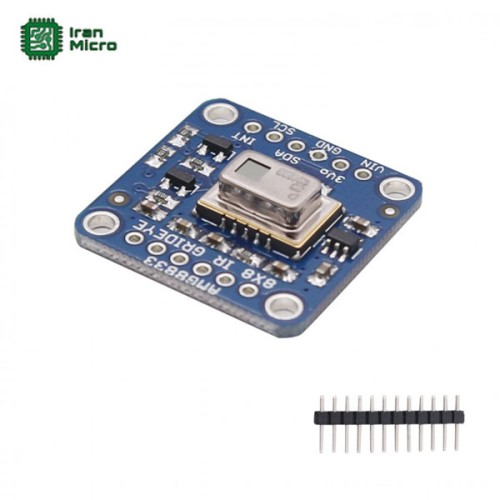
\includegraphics[width=0.5\textwidth]{figs/AMG8833-module-1-500x500 (1).jpg}
	\end{center}
	\caption{\lr{AMG8833}}
\end{figure}


در تصویر زیر نیز می‌توانید نحوه‌ی اتصال این ماژول به رزپری را مشاهده کنید.

\begin{figure}[H]
	\centering
	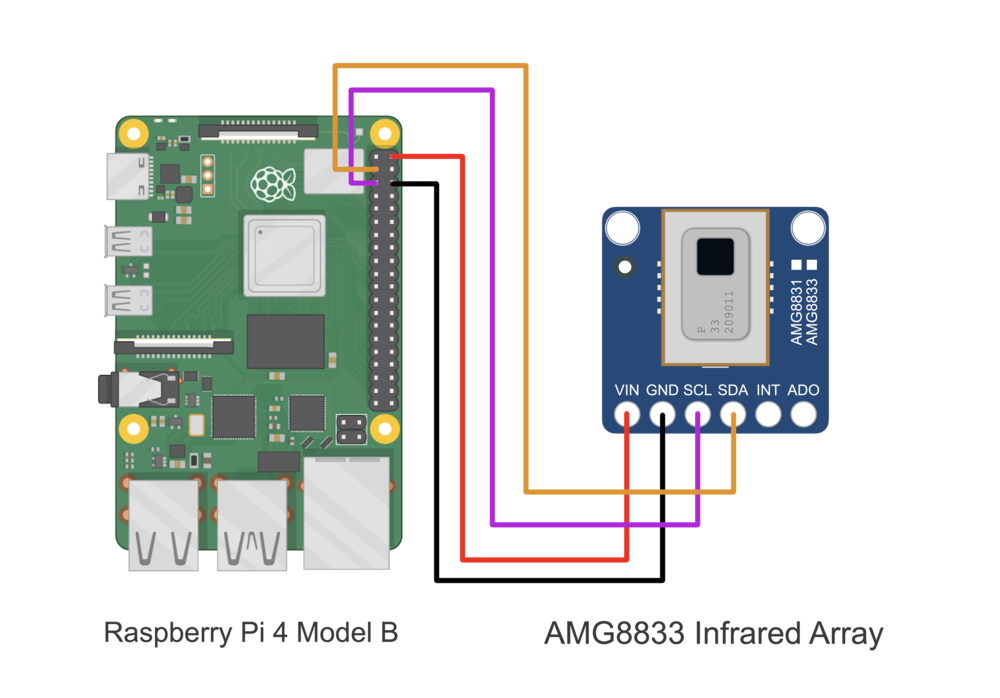
\includegraphics[width=0.5\textwidth]{figs/amg8833_RPi4_wiring.png}
	
	\caption{اتصال سنسور \lr{AMG8833}}
	\label{fig:2}
\end{figure}

همچنین در تصویر زیر می‌توانید یک شماتیک  کلی از نحوه‌ی اتصال کامل مدار ببینید.

\begin{figure}[H]
	\centering
	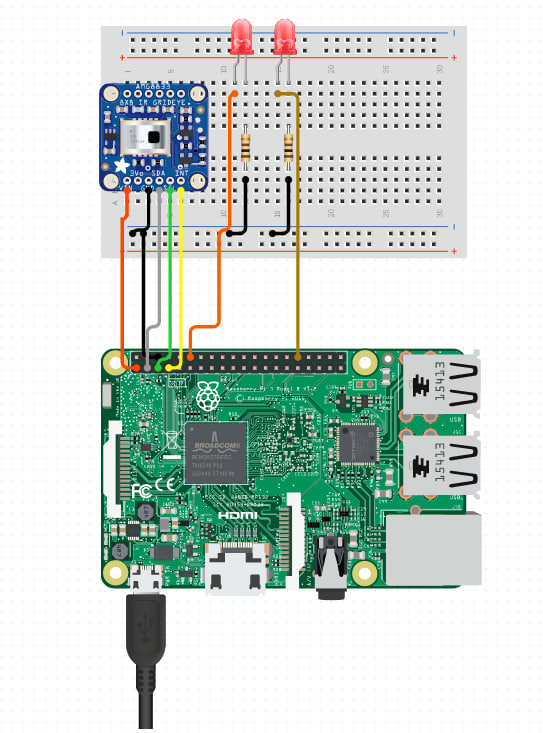
\includegraphics[width=0.5\textwidth]{figs/schematic-overview.jpg}
	
	\caption{شماتیک کلی از مدار}
	\label{fig:2}
\end{figure}

برای خواندن مقادیر از کتاب‌خانه‌ی \lr{smbus}
\footnote{\lr{https://pypi.org/project/smbus2/}}
استفاده شده است. البته این کتابخانه مخصوص این ماژول نمی‌باشد و صرفا خواندن سریال از طریق \lr{i2c} را برایمان راحت کرده است. در نتیجه کد اصلی خواندن دیتا دز دوربین حرارتی پیاده سازی شده است که در ادامه خواهید دید.

بخش‌های مهم پیاده‌سازی مربوط به این قسمت را می‌توانید در زیر مشاهده کنید. (برای جزئیات بیشتر به کد اصلی موجود در ریپازیتوری گیتهاب مراجعه کنید)

\begin{latin}
\begin{lstlisting}[language=python]
import smbus  # i2c bus

class i2c_driver(object):
    
    # Here is the most important function that reads serial
    # data from amg8833 sensor in little_endian order.

    def read16(self, register, little_endian=True):
        # read 16-bits from specified register
        result = self._bus.read_word_data(self._address, register) & 0xFFFF
        if not little_endian:
            result = ((result << 8) & 0xFF00) + (result >> 8)
        return result

    # ...

class AMG8833(object):
    # This important function gets the serial data and converts it 
    # to temperatures in Centigrades. The return value of this function
    # will be an 8x8 matrix.
    
    def read_temp(self, PIXEL_NUM):
        T_arr = []  # temp array
        status = False  # status boolean for errors
        for i in range(0, PIXEL_NUM):
            raw = self.device.read16(GE_PIXEL_BASE + (i << 1))
            converted = self.twos_compl(raw) * 0.25
            if converted < -20 or converted > 100:
                return True, T_arr  # return error if outside temp window
            T_arr.append(converted)
        return status, T_arr



\end{lstlisting}
\end{latin}

در نهایت تابعی که برای خواندن کل آرایه ۸ در ۸ نهایی استفاده می‌شود، تابع \lr{read\_temp} از کلاس تعریف شده در این کد است. این تابع آرایه‌ای شامل ۶۴ عدد \lr{integer} برمی‌گرداند که هر کدام از این اعداد دمای یک پیکسل از ۶۴ پیکسل قابل دید توسط دوربین را نمایش می‌دهد. سپس این آرایه به کمک \lr{numpy} به صورت یک مارتیس ۸ در ۸ در می‌آید که در ادامه خواهیم دید.


\subsection{چراغ‌های \lr{LED}}
با توجه به اینکه اتصال چراغ‌های \lr{LED} تنها نیاز به یک ولتاژ صفر و یک ولتاژ فعال دارد، از توضیح نحوه اتصالشان صرف نظر می‌کنیم. در ادامه‌ می‌توانید کد پیاده‌سازی شده برای روشن یا خاموش کردن چراغ‌ها را مشاهده کنید.

\begin{latin}
\begin{lstlisting}[language=python]
import RPi.GPIO as GPIO

class PinHandler:

    # This class, with its methods, helps us to manage LED lights.
    # Actually makes a wrapper to turn on or off the lights
    # easilly with just a method call.

    @staticmethod
    def left_on():
        GPIO.output(Pin.LEFT.value, GPIO.HIGH)

    @staticmethod
    def left_off():
        GPIO.output(Pin.LEFT.value, GPIO.LOW)

    @staticmethod
    def right_on():
        GPIO.output(Pin.RIGHT.value, GPIO.HIGH)

    @staticmethod
    def right_off():
        GPIO.output(Pin.RIGHT.value, GPIO.LOW)


\end{lstlisting}
\end{latin}

همانطور که در کد می‌توان دید، ۲تابع روشن کردن و ۲تابع خاموش کردن چراغ داریم که هر جفت از خاموش و روشن کردن‌ها مربوط به یکی از جهات راست یا چپ است.

\subsection{بخش نرم افزاری اصلی}
در کنار کد‌های قبلی، یک کد اصلی نیز وجود دارد که مغز متفکر سیستم است و با توجه به شرایط و به تناسب از توابع تعریف شده استفاده می‌کند. در این قسمت بخش‌های مختلف این کد را بررسی‌ می‌کنیم.

در ابتدا کتابخانه‌های مورد نیاز را \lr{import} می‌کنیم. در اینجا از کتابخانه‌ی \lr{logging} برای نگه داشتن تاریخچه‌ی تشخیص‌های سیستم از موجودات زنده استفاده می‌کنیم. همانطور که می‌بینید این تاریخچه در فایلی با اسم \lr{history.log} ذخیره می‌شود.فرمت لاگ خروجی را نیز می‌توانید در زیر ببینید:

\begin{latin}
    2022-12-20 16:07:25,426 - LEFT - 30.0625
\end{latin}

سپس تعداد متغیر اولیه تنظیم شده است که هرکدام استفاده خاص خود را دارند. به عنوان مثال متغیرهای \lr{MIN\_TEMP} و \lr{MAX\_TEMP} بازه‌ی دمایی موجودات زنده را برای سیستم مشخص می‌کند.

\begin{latin}
\begin{lstlisting}[language=python]
import logging
import numpy as np

MIN_TEMP = 29 # Minimum temperature needed to turn on the lights
MAX_TEMP = 50 # Maximum temperature that can be related to a living thing

\end{lstlisting}
\end{latin}

برای تشخیص موجود زنده دو تابع اصلی وجود دارد. در تابع \lr{generate\_submatrices} پنجره‌ای ۲ در ۲ در نظر گرفته می‌شود و این پنجره روی کل ماتریس ۸ در ۸ حاصل از خواندن داده‌های دوربین حرارتی لغزانده می‌شود و روی هر ۴ درایه‌ از این ماتریس که قرار گرفت، میانگین دماهای این ۴ خانه را محاسبه می‌کند. با توجه به اینکه این میانگین در بازه ی تعریف شده وجود دارد یا نه، تشخیص می‌دهد که موجود زنده‌ جلوی سیستم وجود دارد یا خیر. این میانگین‌گیری برای جلوگیری از خطای احتمالی پیکسل‌های جداگانه است تا سیستم منعطف‌تر کار کند و با کوچیکترین تغییر دما واکنش نشان ندهد.
در ادامه می‌توانید کد مربوط به این دو تابع را مشاهده کنید.

\begin{latin}
\begin{lstlisting}[language=python]

def generate_submatrices(matrix, sub_size=2):

    # This function generates all possible NxN submatrices of
    # a given matrix.

    submatrices = []
    for i in range(len(matrix) - sub_size + 1):
        for j in range(len(matrix) - sub_size + 1):
            direction = LEFT

            if j == len(matrix) / 2 - 1:
                direction = MID
            elif j >= len(matrix) / 2:
                direction = RIGHT

            submatrices.append(
                (direction, matrix[i:i + sub_size, j:j + sub_size]))

    return submatrices

def decide_lights(sub_matrices):

    # This function decides which light to turn on
    # based on the location of the high temperature
    # points.

    for direction, sub_matrix in sub_matrices:
        mean = np.mean(sub_matrix)

        if MIN_TEMP <= mean <= MAX_TEMP:
            if direction == LEFT:
                # Turn on the left light
                pin_handler.left_on()
                found_left = True
            elif direction == RIGHT:
                # Turn on the right light
                pin_handler.right_on()
                found_right = True
            elif direction == MID:
                # Turn on both of them
                pin_handler.left_on()
                pin_handler.right_on()
                found_right = True
                found_left = True

    # If there wasn't any living thing on the left side
    # so, turn off the left light
    if not found_left:
        pin_handler.left_off()

    # If there wasn't any living thing on the right side
    # so, turn off the right light
    if not found_right:
        pin_handler.right_off()


\end{lstlisting}
\end{latin}

در تابع \lr{generate\_submatrices} تمام ماتریس‌های ۲ در ۲ ممکن استخراج می‌شود. همچنین در همین تابع تشخیص داده می‌شود که هرکدام از ماتریس‌های ۲ در ۲ تولید شده، در کدام سمت راننده است، در چپ یا راست. این تشخیص جهت به این دلیل است که چراغ درست روشن شود. اگر موجود زنده در سمت راست بود، چراغ راست و اگر در چپ بود چراغ چپ روشن شود. در تابع \lr{decide\_lights} نیز بر اساس داده‌های تولید شده از تابع قبل، تصمیم گرفته می‌شود که کدام چراغ‌ها روشن و یا خاموش شوند. همچنین فرایند ثبت شناسایی‌ها در تاریخچه نیز در همین تابع انجام می‌گیرد. این کار با صدا زدن تابع \lr{log} انجام می‌شود. کد مربوط به این تابع را می‌توانید در زیر ببینید.

\begin{latin}
\begin{lstlisting}[language=python]

def log(direction, mean, sub_matrix):
    # Save any detection of living thing 

    logging.info(f"{direction} - {mean} - {sub_matrix}")

\end{lstlisting}
\end{latin}

در نهایت یک تابع \lr{main} وجود دارد که در یک حلقه‌ی بینهایت مقادیر دوربین حرارتی را خوانده و توابع تعریف شده در بالا را صدا می‌زند. این کد را می‌توانید در زیر مشاهده کنید:

\begin{latin}
\begin{lstlisting}[language=python]

def main():
    # This function acts as a coordinator that calls
    # all needed functions to read data from sensor
    # and decide to turn on the correct light based
    # on the position of the detected living thing.

    t0 = time.time()
    sensor = []

    while (time.time() - t0) < 1:
        sensor = amg8833_i2c.AMG8833(addr=0x69)

    pixels_resolution = (8, 8)
    pixels_to_read = 64

    while True:
        # Read serial data from sensor
        status, pixels = sensor.read_temp(pixels_to_read)
        if status:
            continue

        # The temperature of the thermistor used in the sensor
        T_thermistor = sensor.read_thermistor()

        # Trasnforming sensor serial data to an 8x8 numpy array
        pixels_reshaped = np.reshape(pixels, pixels_resolution)

        # Generate all 2x2 submatrices
        submatrices = generate_submatrices(pixels_reshaped)
        
        # Turn on/off the lights based on the values of sensor's data
        decide_lights(submatrices)

if __name__ == '__main__':
    main()

\end{lstlisting}
\end{latin}

در این تابع ابتدا دوربین حرارتی اتصالش برقرار شده سپس همواره ۶۴ پیکسل از آن خوانده می‌شود و به صورت یک ماتریس ۸ در ۸ تبدیل می‌شود. سپس ماتریس‌های ۲ در ۲ تولید شده از آن به تابع \lr{decide\_lights} داده می‌شود تا تصمیمگیری‌های مربوط به چراغ‌ها را انجام دهد. این فرایند تا زمان خرابی سیستم یا قطع آن توسط کاربر انجام خواهد شد.



\subsection{بسته بندی}
این قسمت هنوز طراحی نشده است.



\chapter{خروجی}
در این قسمت خروجی دستگاه را طی چند اجرای نمونه بررسی ‌می‌کنیم.

\section{تست در روشنایی}

در تصویر زیر می‌توانید مشاهده کنید که چرا سمت چپ خودرو در حضور یک منبع حرارتی جلوی سنسور روشن شده است. همچنین این منبع در سمت چپ خودرو قرار دارد. 

\begin{figure}[H]
	\centering
	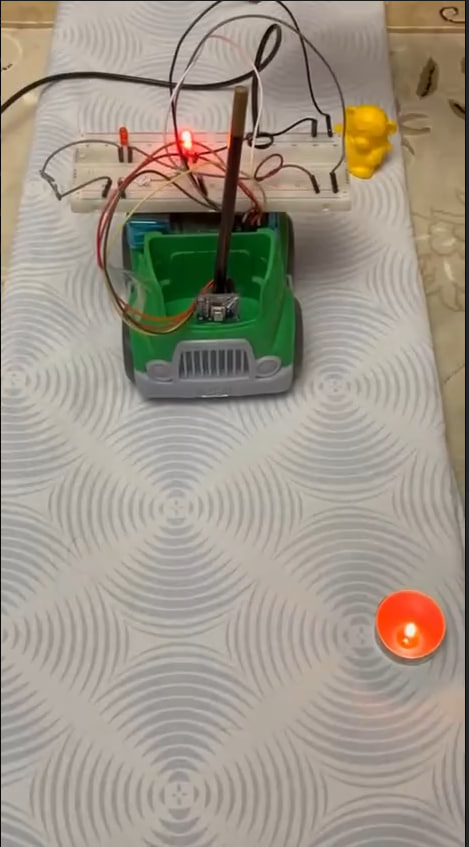
\includegraphics[width=0.5\textwidth]{figs/test_with_lights_on.jpg}
	\caption{تست در روشنایی}
	\label{fig:2}
\end{figure}

در زیر می‌توانید مقداری که اجرای کد، در خروجی استاندار (\lr{stdout}) خود نمایش می‌دهد قبل و بعد از روشن شدن چراغ مشاهده کنید.


آرایه خروجی زیر، قبل از قرار گرفتن شمع در برابر خودرو است. همانطور که می‌بینید تمام دماها‌ی نشان داده شده برای هر پیکسل، تقریبا برابر همان دمای محیط است.
\begin{latin}
\begin{lstlisting}[language=python]
[[23.1 24.4 24.4 23.2 24.7 23.6 23.8 23.8]
 [24.1 24.4 24.9 23.7 24.8 23.5 23.9 23.3]
 [23.6 24.  24.7 24.3 24.7 24.9 24.7 24. ]
 [24.9 23.2 23.7 24.9 24.3 23.6 23.9 23.7]
 [23.3 24.  23.  24.9 24.8 24.2 23.7 23.9]
 [23.8 23.6 23.  23.3 24.9 24.1 24.6 23.6]
 [23.3 23.5 24.8 23.3 23.3 24.2 24.  24.9]
 [23.  23.2 24.7 23.  24.3 23.9 23.  24.6]]
\end{lstlisting}
\end{latin}

اما پس از قرار گیری منبع گرما در برابر خودرو، تغییری ملموس در سمت راست ماتریس خروجی مشاهده می‌شود که نشان از افزایش دما در ناحیه خاصی از محیط دارد. این تغییر دما به احتما قوی می‌تواند مربوط به حضور یک موجود زنده در جلوی خودرو باشد. پس در همین زمان است که دستگاه با روشن کردن چراغ سمت چپ، به راننده هشدار می‌دهد که موجودی زنده در سمت چپ او قرار دارد.
\begin{latin}
\begin{lstlisting}[language=python]
[[23.8 24.8 24.2 24.4 23.4 39.6 40.4 40.2]
 [23.3 23.4 24.4 23.4 23.5 40.4 39.9 39.9]
 [24.6 23.8 23.6 24.2 24.8 39.2 40.4 39. ]
 [23.  24.2 24.9 24.5 23.  47.3 39.2 49.8]
 [23.5 24.  24.1 23.8 24.5 49.9 40.2 48.5]
 [23.4 24.2 24.4 24.4 23.4 39.  40.9 39.3]
 [23.6 23.6 23.7 24.2 23.2 40.6 39.9 39.5]
 [23.5 24.4 23.5 24.8 23.1 40.3 39.7 40.1]]
\end{lstlisting}
\end{latin}


\section{تست در تاریکی}

در تصویر زیر می‌توانید مشاهده کنید که چرا سمت راست خودرو در حضور یک منبع حرارتی جلوی سنسور روشن شده است. همچنین این منبع در سمت راست خودرو قرار دارد. 

\begin{figure}[H]
	\centering
	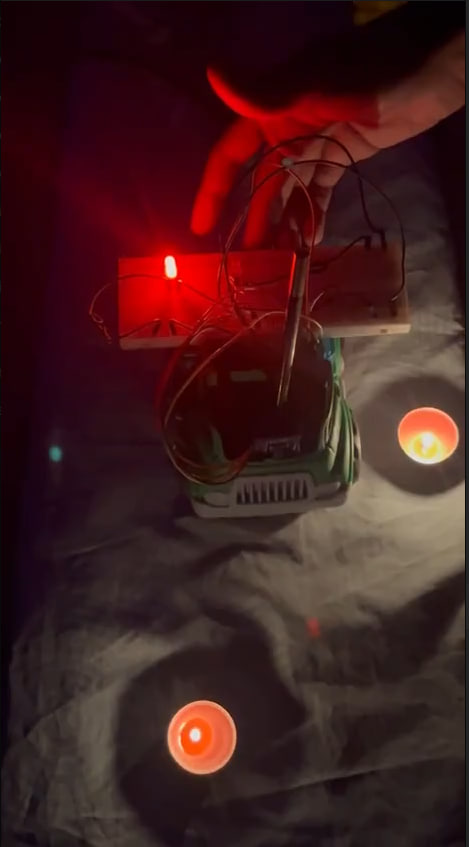
\includegraphics[width=0.5\textwidth]{figs/test_with_lights_off.jpg}
	\caption{تست در تاریکی}
	\label{fig:2}
\end{figure}

در زیر می‌توانید مقداری که اجرای کد، در خروجی استاندار (\lr{stdout}) خود نمایش می‌دهد قبل و بعد از روشن شدن چراغ مشاهده کنید.


آرایه خروجی زیر، قبل از قرار گرفتن شمع در برابر خودرو است. همانطور که می‌بینید تمام دماها‌ی نشان داده شده برای هر پیکسل، تقریبا برابر همان دمای محیط است.
\begin{latin}
\begin{lstlisting}[language=python]
[[23.1 23.  23.7 24.3 24.1 24.7 24.2 23.4]
 [24.2 23.4 24.  24.5 24.7 23.1 23.9 24.9]
 [24.4 23.3 24.9 24.9 24.4 24.9 23.6 23.1]
 [24.4 23.7 23.4 24.7 23.9 24.3 23.6 23.3]
 [24.4 24.3 23.3 23.1 24.2 23.9 23.5 23.4]
 [23.5 23.2 24.8 23.8 23.5 23.7 23.7 24.1]
 [23.6 23.7 23.5 24.5 23.1 23.8 24.6 23. ]
 [24.1 24.2 24.2 24.4 23.2 24.1 24.4 24. ]]
\end{lstlisting}
\end{latin}

اما پس از قرار گیری منبع گرما در برابر خودرو، تغییری ملموس در سمت چپ ماتریس خروجی مشاهده می‌شود که نشان از افزایش دما در ناحیه خاصی از محیط دارد. این تغییر دما به احتما قوی می‌تواند مربوط به حضور یک موجود زنده در جلوی خودرو باشد. پس در همین زمان است که دستگاه با روشن کردن چراغ سمت راست، به راننده هشدار می‌دهد که موجودی زنده در سمت راست او قرار دارد.
\begin{latin}
\begin{lstlisting}[language=python]
[[45.1 45.  45.7 46.3 24.1 24.7 24.2 23.4]
 [46.2 45.4 46.  46.5 24.7 23.1 23.9 24.9]
 [46.4 45.3 46.9 46.9 24.4 24.9 23.6 23.1]
 [51.4 50.7 45.4 46.7 23.9 24.3 23.6 23.3]
 [54.4 53.3 45.3 45.1 24.2 23.9 23.5 23.4]
 [45.5 45.2 46.8 45.8 23.5 23.7 23.7 24.1]
 [45.6 45.7 45.5 46.5 23.1 23.8 24.6 23. ]
 [46.1 46.2 46.2 46.4 23.2 24.1 24.4 24. ]]
\end{lstlisting}
\end{latin}



